% ----------------------------------------------------------------------
% Template VERIFICA
% ----------------------------------------------------------------------
% 2020 di d!egofantinelli at jazzmagus@gmail.com
% ----------------------------------------------------------------------

% ---------------------------------- Preambolo
\documentclass[11pt, a4paper]{exam}
\usepackage[T1]{fontenc}
\usepackage{mdframed}
%\usepackage{nicefrac}
%\usepackage[applemac]{inputenc}
%\usepackage[utf8]{inputenc}
\usepackage[italian]{babel}
\usepackage[margin=1.3in]{geometry}
\usepackage{amsmath,amssymb}
\usepackage{multicol}
\usepackage{graphicx}
\usepackage{tikz}
\usepackage{upquote}
\usepackage{caption}
%\usepackage{fancyhdr}
\usepackage{float}

%\printanswers

% ---------------------------------- Command
\renewcommand{\questionshook}{%
    \setlength{\leftmargin}{0pt}%
}
\renewcommand{\choiceshook}{%
    \setlength{\leftmargin}{20pt}%
}

\newcommand{\class}{\huge {Verifica di Matematica}}
\newcommand{\term}{Recupero Primo Quadrimestre}
%\newcommand{\examnum}{Verifica numero: 1}
\newcommand{\examdate}{25 febbraio 2021}
\newcommand{\timelimit}{40 minuti}

\CorrectChoiceEmphasis{\color{red}}
\SolutionEmphasis{\color{red} \footnotesize}
\renewcommand{\solutiontitle}{\noindent\textbf{Soluzione:}\par\noindent}

% ---------------------------------- Headers and Footers

\pagestyle{headandfoot}
\firstpageheader{IIS "G. A. Remondini" - Bassano del Grappa (VI)}{}{\examdate}
\runningheader{\footnotesize VERIFICA di Recupero di MATEMATICA}{}{Classe 5\string^QA}
\runningheadrule

\firstpagefooter{}{}{pag. \thepage\ di \numpages}
\runningfooter{}{}{pag. \thepage\ di \numpages}
\runningfootrule

% ---------------------------------- Punteggi
\pointpoints{punto}{\em punti}
\pointformat{[{\footnotesize \thepoints}]}
\bonuspointpoints{punto bonus}{\em punti bonus}
\bonuspointformat{[{\footnotesize \thepoints}]}
\pointsinrightmargin
\setlength{\rightpointsmargin}{.2cm}
\chqword{Esercizio}
\chpword{Punti}
\chbpword{Punti Bonus}
\chsword{Punteggio}
\chtword{Totale}

\begin{document}

% ---------------------------------- Title Page
\begin{center}
\rule[2ex]{\textwidth}{0.5pt}\\
{\huge{\bf \class}}\\[12pt]
{\huge -\, \term \, - }\\[8pt]
\rule[2ex]{\textwidth}{0.5pt}\\
\end{center}
\vspace{3cm}
\begin{tabular*}{\textwidth}{l @{\extracolsep{\fill}} r @{\extracolsep{6pt}} l}
\textbf{} & \textbf{Nome e Cognome:} & \makebox[2.5in]{\hrulefill}\\
\textbf{} &&\\
\textbf{} & \textbf{Classe:} & \makebox[2.5in]{\Large{\bf 5 \string^ QA}}\\
\textbf{} &&\\
\textbf{} & Tempo a disposizione: & \makebox[2.5in]{\timelimit}
\end{tabular*}\\[3cm]
\vspace{5cm}
% ---------------------------------- Avvertenze

\noindent
%\rule[2ex]{\textwidth}{0.2pt}
\textbf{Avvertenze}:
\begin{itemize}
	\item La presente Verifica - che viene somministrata in modalit� DDI - contiene \numquestions \; quesiti, per un totale di \numpoints \;punti.
	\item La webcam dovr� rimanere accesa per tutto il tempo della verifica (\timelimit), salvo impossibilit� concrete di connessione; il microfono rester� spento e verr� acceso soltanto per chiarimenti e domande, che saranno consentite negli ultimi 20 min della prova.
	\item E' vietato l'utilizzo di calcolatrici scientifiche, smartphone, tablet e altri dispositivi digitali, nonch� la consultazione di testi, appunti e siti web.

\end{itemize}%\rule[2ex]{\textwidth}{0.2pt}
\vfill
\newpage

% ---------------------------------- Esercizi0 1

\begin{questions}

\addpoints
\question
Determinare l'Insieme di Definizione delle seguenti Funzioni \((f : x \in \mathbb{R} \to  y \in \mathbb{R})\), e classificarle in base alla tipologia:\\
\begin{parts}
\part[4]
\( y= f(x) = {\dfrac{2x}{x^2 - 4}}\)\\
\fillwithlines{0.5in}
{\footnotesize
\begin{solution}
Funzione algebrica Razionale Fratta\\
	\(D=\{x \in \mathbb{R} : x \neq \pm 2\}\)
\end{solution}
}
\vspace{.5cm}

\part[5]
\( y= f(x) = \dfrac{1}{x^2} - \dfrac{1}{3x - 9}\)\\
\fillwithlines{0.5in}
{\footnotesize
\begin{solution}
Funzione algebrica Razionale Fratta\\
	\(D = \{x \in \mathbb{R} : x \neq 0 \lor x \neq 3\}\)
\end{solution}
}
\vspace{.5cm}

\part[6]
\( y= f(x) = {\dfrac{x}{\sqrt{x^2 - 4}}}\)\\
\fillwithlines{0.5in}
{\footnotesize
\begin{solution}
Funzione algebrica Irrazionale Fratta\\
	\(D = \{x \in \mathbb{R} : x < - 2 \lor x > 2\}\)
\end{solution}
}

\end{parts}
\vspace{.8cm}

%------------------------------------------- Esercizio 2
\addpoints
\question [6] Qual � l'Insieme di Definizione della seguente funzione? \[y= f(x) = {\dfrac{\sqrt {x - 1}}{x^2 + 3x + 4}}\]

\begin{choices}
\setlength{\leftmargin}{0pt}
 \choice \(D = \{x \in \mathbb{R}\}\)
 \choice \(D = \{x \in \mathbb{R} : x \neq \pm 1\}\)
 \CorrectChoice \(D = \{x \in \mathbb{R} : x \ge 1\}\)
 \choice \(D = \{x \in \mathbb{R} : x \neq 0; \, x \neq 1\}\)
 
\end{choices}
\vspace{.8cm}

%------------------------------------------- Esercizio 3
\addpoints
\question [4] Quale delle seguenti funzioni {\bf non} ha come Insieme di Definizione ? \[D = \{x \in \mathbb{R} \}\]

\begin{choices}
\setlength{\leftmargin}{0pt}
 \choice \(y = f(x) = x^2 - \dfrac{1}{2}x\)
 \CorrectChoice\(y = f(x) = \dfrac{1}{2x^2 - 1}\)
 \choice \(y = f(x) = \dfrac{1}{2x^2 + 1}\)
 \choice \(y = f(x) = x^2 - \dfrac{1}{2}x\)

\end{choices}
\vspace{.8cm}

\pagebreak
%------------------------------------------- Esercizio 4
\addpoints
\question[5] 

Determina l'Insieme di Definizione e le Intersezioni con gli assi della funzione il cui grafico � riportato in figura; utilizza il grafico per verificare la correttezza dei risultati: \[y = f(x) = \dfrac{x^2 - 4}{1 - x^3}\]\\

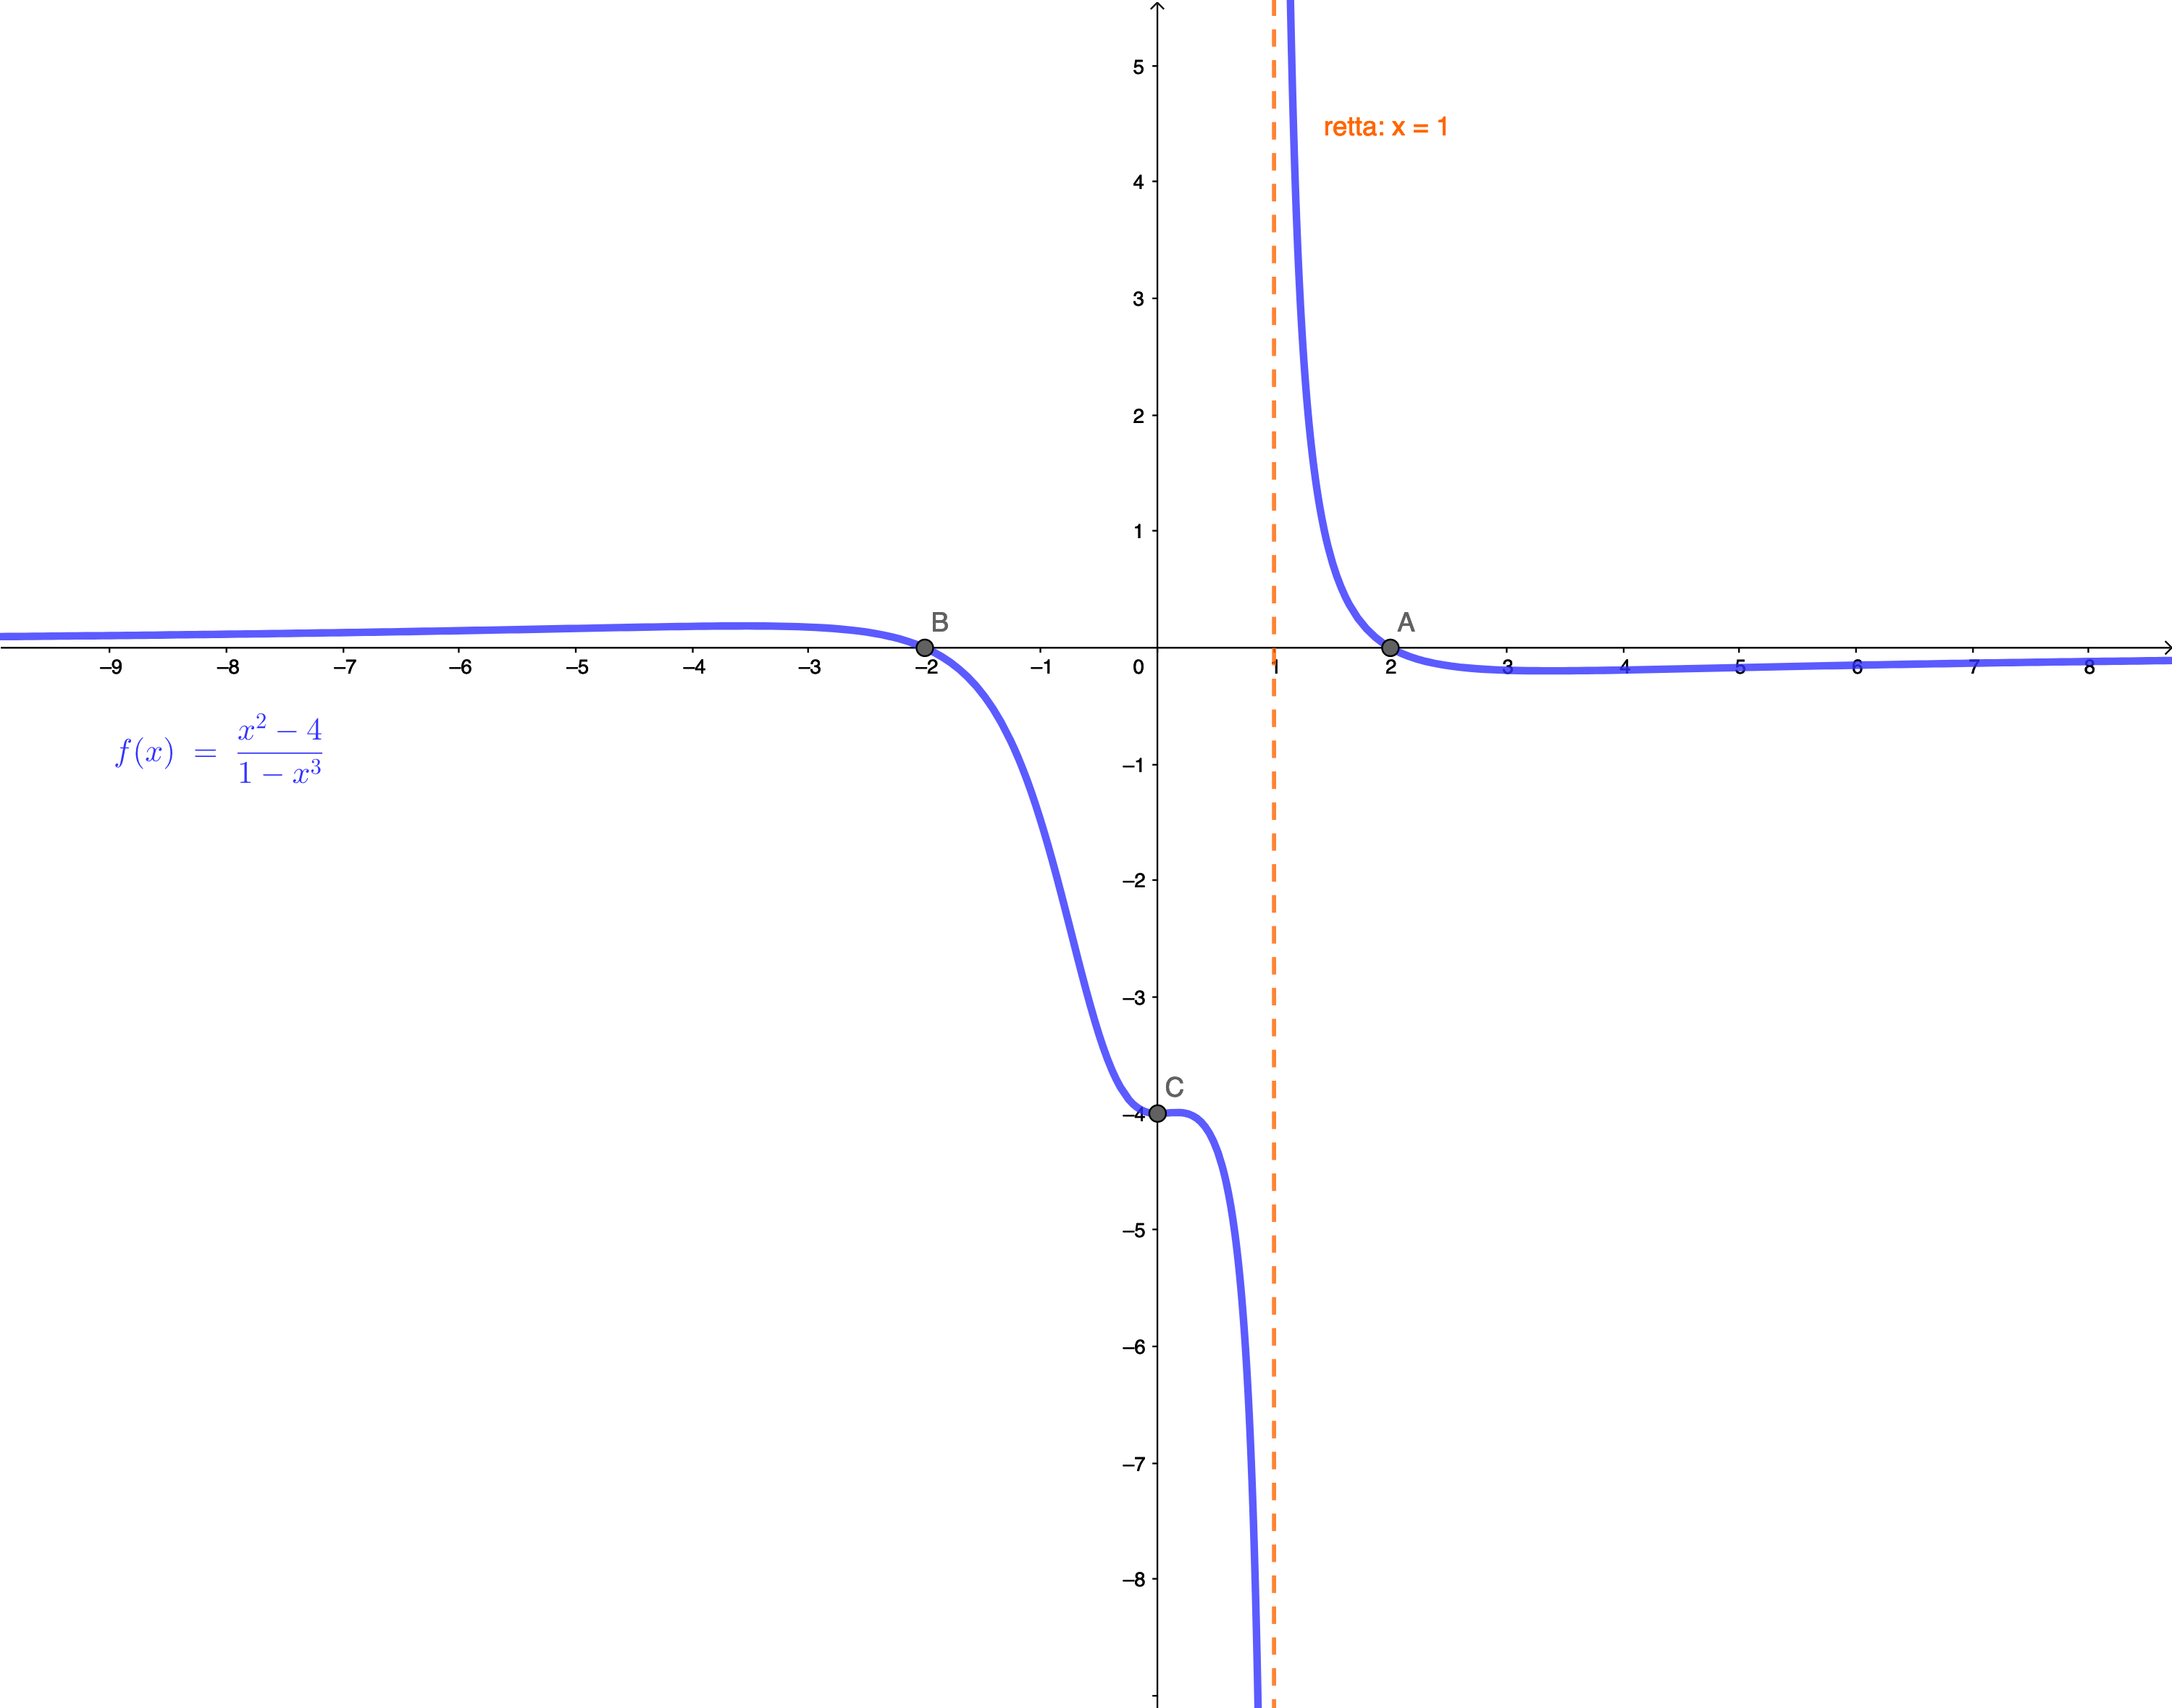
\includegraphics[width=\textwidth]{funzione}
{\footnotesize
\begin{solution}
	\(D = \{x \in \mathbb{R} : x \neq 1\}; \quad A(2, 0); \quad B(0, -2); \quad C(-4, 0)\)
\end{solution}
}
\fillwithlines{0.75in}
\end{questions}

\vfill
\noindent
\rule[2ex]{\textwidth}{1pt}

%\pagebreak
\begin{center}
{\bf Tabella dei punteggi}
\vspace{10pt}

\combinedgradetable[h][questions]
\end{center}
\vspace{8pt}
\footnotesize La sufficienza � fissata a 18 punti, ma potr� subire delle modifiche in fase di correzione, al fine di garantire la validit� della prova anche nel caso in cui si riscontrassero prestazioni della classe sensibilmente lontane dalla media-classe stimata.

\end{document}
